\documentclass[14pt,hidelinks]{extarticle}

%%% Поля и разметка страницы %%%
\usepackage{pdflscape}   % Для включения альбомных страниц
\usepackage{geometry} % Для последующего задания полей
\usepackage{setspace} % Для интерлиньяжа
\usepackage[14pt]{extsizes}
\usepackage{titlesec}
\usepackage{tocloft}
\usepackage{enumitem}
\usepackage{fancyhdr}

%%% Кодировки и шрифты %%%
\usepackage{cmap}                    % Улучшенный поиск русских слов в полученном pdf-файле
\usepackage[T2A]{fontenc}	     % Поддержка русских букв
\usepackage[utf8]{inputenc}	     % Кодировка utf8
\usepackage[english=nohyphenation,russian=nohyphenation]{hyphsubst} % Запрет переносов
\usepackage[english, russian]{babel} % Языки: русский, английский
% \usepackage{pscyr}						% Красивые русские шрифты

%%% Математические пакеты %%%
\usepackage{amsthm,amsfonts,amsmath,amssymb,amscd} % Математические дополнения от AMS

%%% Оформление абзацев %%%
\usepackage{indentfirst} % Красная строка

%%% Цвета %%%
\usepackage[usenames]{color}
\usepackage{color}
\usepackage{colortbl}

%%% Таблицы %%%
\usepackage{longtable}		     % Длинные таблицы
\usepackage{multirow,makecell,array} % Улучшенное форматирование таблиц

%%% Общее форматирование
\usepackage{caption}
\captionsetup[figure]{labelsep=space,justification=centering,singlelinecheck=false}
\captionsetup[lstlisting]{labelsep=space,justification=centering,singlelinecheck=false}

\usepackage{soul}                    % Поддержка переносоустойчивых подчёркиваний и зачёркиваний
\usepackage{multicol}

%%% Библиография %%%
\usepackage{cite} % Красивые ссылки на литературу

%%% Гиперссылки %%%
\usepackage[unicode,plainpages=false,pdfpagelabels=false]{hyperref}

%%% Изображения %%%
\usepackage{graphicx} % Подключаем пакет работы с графикой     % Подключаемые пакеты
%%% Макет страницы %%%
\geometry{a4paper,top=20mm,bottom=27mm,left=30mm,right=15mm}
\onehalfspacing
%%% Язык текста %%%
\selectlanguage{russian}

%%% Кодировки и шрифты %%%
\renewcommand{\rmdefault}{ftm} % Включаем Times New Roman

%%% Выравнивание и переносы %%%
\sloppy				% Избавляемся от переполнений
\clubpenalty=10000		% Запрещаем разрыв страницы после первой строки абзаца
\widowpenalty=10000		% Запрещаем разрыв страницы после последней строки абзаца
\interfootnotelinepenalty=10000 % запрет разрыва сносок

%%% Нумерация %%%

\fancyhf{}
\renewcommand{\headrulewidth}{0pt}
\rfoot{\thepage}
\pagestyle{fancy}

%%% Библиография %%%
\makeatletter
\bibliographystyle{utf8gost705u}	% Оформляем библиографию в соответствии с ГОСТ 7.0.5

%%% Изображения %%%
\graphicspath{{images/}} % Пути к изображениям

%%% Содержание %%%
\renewcommand{\cfttoctitlefont}{\hfil\large\bfseries}
\renewcommand\cftsecfont{\normalsize}
\renewcommand\cftsecpagefont{\normalsize}
\renewcommand{\cftsecleader}{\cftdotfill{\cftdotsep}}
\setlength\cftparskip{0pt}
\setlength\cftbeforesecskip{0pt}
\setlength\cftaftertoctitleskip{14pt}

\setlength{\cftsecindent}{0ex}
\setlength{\cftsubsecnumwidth}{5ex}

\setlength{\cftsecnumwidth}{2ex}
\setlength{\cftsubsecnumwidth}{4ex}

%%% Требования ЕСКД/СТП %%%

%%% Размеры заголовков
\titleformat{\section}{\large\bfseries}{\thesection}{1ex}{}
\titleformat{name=\section,numberless}{\large\bfseries\filcenter}{}{1ex}{}
\titlespacing*{\section}{5ex}{14pt}{14pt}

\titleformat{name=\subsection}{\normalsize\bfseries}{\thesubsection}{1ex}{}
\titleformat{name=\subsection,numberless}{\normalsize\bfseries}{}{1ex}{}
\titlespacing*{\subsection}{5ex}{14pt}{14pt}

%%% Размеры текста формул %%%
\DeclareMathSizes{12}{12}{6}{4}

%%% Оформление текста
\setlength{\topskip}{14pt}

\setlength{\parskip}{0pt}
\setlength{\parindent}{5ex}

\setlength{\floatsep}{14pt}
\setlength{\textfloatsep}{14pt}
\setlength{\intextsep}{14pt}
\setlength{\abovecaptionskip}{14pt}
\setlength{\belowcaptionskip}{0pt}

\setlength{\topsep}{0pt}
\setlength{\partopsep}{0pt}
\setlength{\itemsep}{0pt}

\expandafter\def\expandafter\normalsize\expandafter{%
  \normalsize
  \setlength{\abovedisplayskip}{14pt}
  \setlength{\abovedisplayshortskip}{0pt}
  \setlength{\belowdisplayskip}{14pt}
  \setlength{\belowdisplayshortskip}{14pt}
}
% \setlength{}{}                  
\setitemize[0]{leftmargin=7.5ex,itemsep=0pt,topsep=0pt,parsep=0pt}
\renewcommand{\labelitemi}{$-$}

%\numberwithin{equation}{section}
%\renewcommand{\thefigure}{\thesection.\arabic{figure}}
\captionsetup[figure]{labelsep=endash,singlelinecheck=false,skip=0em}
%\renewcommand{\labelenumi}{\thesection.\arabic{enumi}. }

%\renewcommand{\thetable}{\thesection.\arabic{table}} 
\captionsetup[table]{labelsep=endash,justification=raggedright,singlelinecheck=false,skip=0em}
\renewcommand{\arraystretch}{1.1}

%%% Красоты %%%	     % Пользовательские стили

\begin{document}

%%% Переопределение именований %%%
\renewcommand{\abstractname}{Аннотация}
\renewcommand{\alsoname}{см. также}
\renewcommand{\appendixname}{Приложение}
\renewcommand{\bibname}{Литература}
\renewcommand{\ccname}{исх.}
\renewcommand{\chaptername}{Глава}
\renewcommand{\contentsname}{СОДЕРЖАНИЕ}
\renewcommand{\enclname}{вкл.}
\renewcommand{\figurename}{Рисунок}
\renewcommand{\headtoname}{вх.}
\renewcommand{\indexname}{Предметный указатель}
\renewcommand{\listfigurename}{Список рисунков}
\renewcommand{\listtablename}{Список таблиц}
\renewcommand{\pagename}{Стр.}
\renewcommand{\partname}{Часть}
\renewcommand{\seename}{см.}
\renewcommand{\tablename}{Таблица}

\renewcommand{\refname}{СПИСОК ИСПОЛЬЗОВАННЫХ ИСТОЧНИКОВ}	     % Переопределение именований

%%%%%%%%%%%%%%%%%%%%%%%%%%%%%%%%%%%%%%%%%%%%%%%%%%%%%%%%%%%%%%%%

\begin{center}
	\textbf{Типовой расчет} \\ 
	выполнил ст. гр. ****** Ю.А. Петров \\
        Задача №10\\
	Вариант XX 
\end{center}

\section{Условие}

По выборке одномерной случайной величины:

\begin{itemize}
	\item получить вариационный ряд;
	\item построить на масштабно-координатной бумаге формата А4 график эмпирической функции распределения $ F^*(x) $; 
	\item построить гистограмму равноинтервальным способом;
	\item вычислить оценки математического ожидания и дисперсии при заданном значении надежности;
	\item выдвинуть гипотезу о законе распределения случайной величины и проверить её при помощи критерия согласия $ \chi^2 $ и критерия Колмогорова ($ \alpha = 0,05 $).
\end{itemize}

Вариационный ряд исходной выборки приведен в таблице~\ref{tbl:first_sample}.

\renewcommand{\tabcolsep}{0.6em} 
\begin{table}[h!]
	\centering
	\caption{Одномерная выборка\label{tbl:first_sample}}
	\label{tbl:first}
	\begin{tabular}{cccccccccc}
		(-0.68; -0.26)	& (-4.03; -2.32)	& (-0.72; 0.47)	& (1.25; 0.82)	& (1.27; -0.81)	\\ 
(-3.57; 0.46)	& (3.00; -2.85)	& (-2.19; 2.71)	& (-4.72; 0.48)	& (4.38; 2.77)	\\ 
(1.16; 2.37)	& (-1.04; 2.03)	& (-0.63; 1.74)	& (-0.07; -0.30)	& (-1.55; 1.85)	\\ 
(1.57; -0.10)	& (-0.27; -0.84)	& (-1.92; -0.17)	& (-0.80; -0.27)	& (-0.30; 3.87)	\\ 
(-2.51; -1.20)	& (0.21; 0.36)	& (2.99; 2.78)	& (2.26; 2.43)	& (1.95; 0.79)	\\ 
(3.27; 0.62)	& (-0.40; 2.71)	& (-0.53; 1.01)	& (0.16; 2.11)	& (3.07; 0.47)	\\ 
(-0.87; -2.17)	& (2.41; -0.85)	& (-0.52; -1.54)	& (0.99; -0.26)	& (0.57; 1.41)	\\ 
(1.47; -0.41)	& (5.76; -1.11)	& (-1.16; 0.95)	& (-1.22; -3.60)	& (3.13; 2.46)	\\ 
(0.90; 0.79)	& (0.77; -3.32)	& (-0.80; -1.46)	& (1.48; -0.69)	& (0.18; 0.25)	\\ 
(2.08; 2.50)	& (-0.99; -2.73)	& (-1.33; 1.70)	& (-2.36; -2.75)	& (-1.82; -2.29)	\\ 
	\\ 

	\end{tabular}
\end{table}

\newpage

\section{Решение}

\subsection{Построение эмпирической функции распределения $F^*(x)$}
Для построения эмпирической функции распределения $F^*(x)$ необходимо воспользоваться следующей формулой:
\begin{equation}
	\begin{aligned}
		F^*(x)=p^*(X<x)=
		\left\{
			\begin{aligned}
				&0, \hspace{5mm} x \le \hat{x}_1, \\
				&\vdots \\
				&\frac{i}{n}, \hspace{4mm} \hat{x}_i < x \le \hat{x}_{i+1}, \\
				&\vdots \\
				&1, \hspace{5mm} x > \hat{x}_n.
			\end{aligned}
		\right.
	\end{aligned}
\end{equation}

График эмпирической функции распределения $F^*(x)$ приведен на рисунке~\ref{fig:emp_distrib}.
\begin{figure}[h!] 

  \centering
  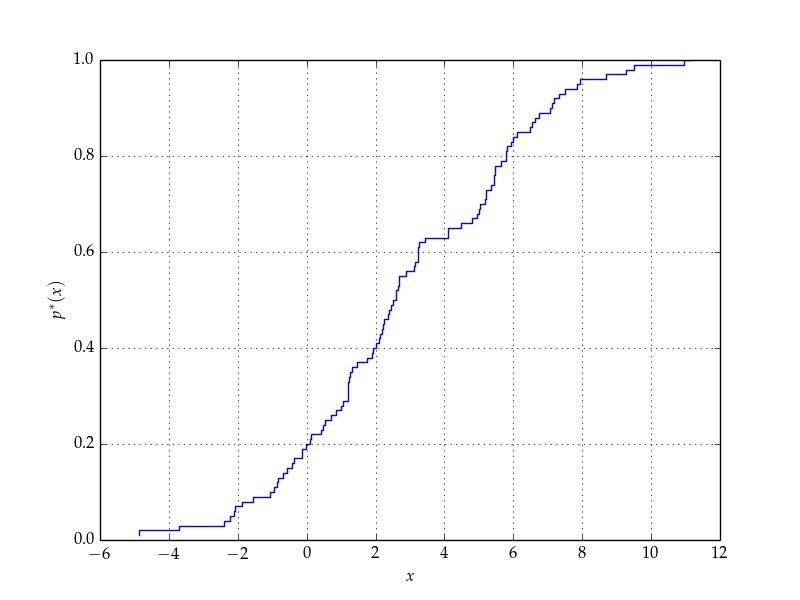
\includegraphics[width=1\linewidth]{pic/sample.png}
  \caption{График эмпирической функции распределения $F^*(x)$\label{fig:emp_distrib}}
\end{figure}

\newpage

\subsection{Построение гистограмм}

Вычислим значения интервального статистического ряда (таблица~\ref{tabl:eq-size_int}) для построения
равноинтервальной гистограммы (рисунок~\ref{fig:eq-size_hist}).

\renewcommand{\tabcolsep}{1.5em} 
\begin{table}[h!]
  \centering
  \caption{Равноинтервальный статистический ряд\label{tabl:eq-size_int}}
  \small
  \begin{tabular}{|c|c|c|c|c|c|c|}
    \hline
    $ j $	& $ A_j $	& $ B_j $	& $ h_j $	& $ v_j $	& $ p^{*}_j $	& $ f^{*}_j $ \\ \hline
1	& -4.860	& -3.259	& 1.601	& 2	& 0.0200	& 0.0125 \\ \hline
2	& -3.259	& -1.658	& 1.601	& 5	& 0.0500	& 0.0312 \\ \hline
3	& -1.658	& -0.057	& 1.601	& 11	& 0.1100	& 0.0687 \\ \hline
4	& -0.057	& 1.544	& 1.601	& 18	& 0.1800	& 0.1124 \\ \hline
5	& 1.544	& 3.145	& 1.601	& 20	& 0.2000	& 0.1249 \\ \hline
6	& 3.145	& 4.746	& 1.601	& 9	& 0.0900	& 0.0562 \\ \hline
7	& 4.746	& 6.347	& 1.601	& 19	& 0.1900	& 0.1187 \\ \hline
8	& 6.347	& 7.948	& 1.601	& 11	& 0.1100	& 0.0687 \\ \hline
9	& 7.948	& 9.549	& 1.601	& 3	& 0.0300	& 0.0187 \\ \hline
10	& 9.549	& 11.150	& 1.601	& 2	& 0.0200	& 0.0125 \\ \hline
Всего:	&	&	&16.010	&100	&1.0000	& \\ \hline

  \end{tabular}
\end{table}

\begin{figure}[h!]
  \centering
  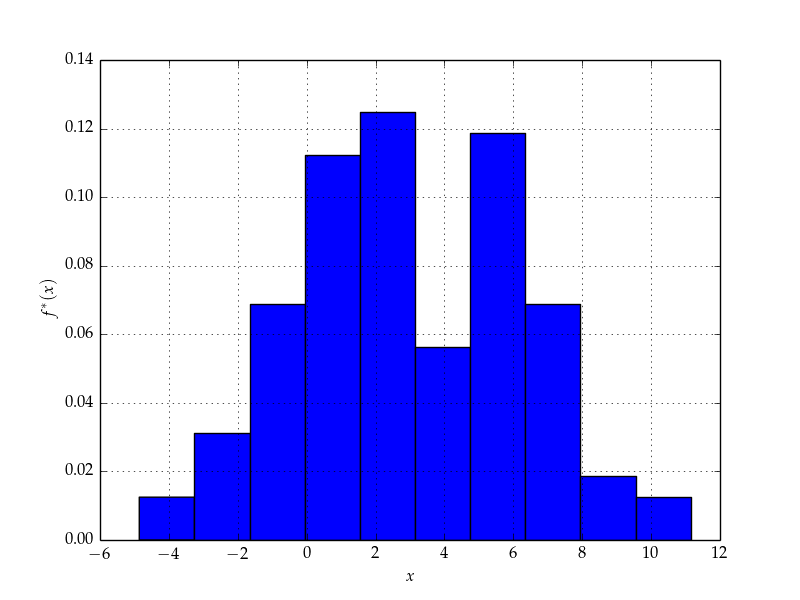
\includegraphics[width=1\linewidth]{pic/stat_series_eq_size.png}
  \caption{Равноинтервальная гистограмма распределения случайной величины $ X $\label{fig:eq-size_hist}}
\end{figure}

Вычислим значения интервального статистического ряда (таблица~\ref{tabl:eq-prob_int}) для построения
равновероятностной гистограммы (рисунок~\ref{fig:eq-prob_hist}).
\begin{table}[h!]
	\centering
	\caption{Равновероятностный статистический ряд\label{tabl:eq-prob_int}}
        \small
	\begin{tabular}{|c|c|c|c|c|c|c|}
		\hline
		$ j $	& $ A_j $	& $ B_j $	& $ h_j $	& $ v_j $	& $ p^{*}_j $	& $ f^{*}_j $ \\ \hline
1	& -4.860	& -0.905	& 3.955	& 10	& 0.1000	& 0.0253 \\ \hline
2	& -0.905	& 0.115	& 1.020	& 10	& 0.1000	& 0.0980 \\ \hline
3	& 0.115	& 1.210	& 1.095	& 10	& 0.1000	& 0.0913 \\ \hline
4	& 1.210	& 2.055	& 0.845	& 10	& 0.1000	& 0.1183 \\ \hline
5	& 2.055	& 2.600	& 0.545	& 10	& 0.1000	& 0.1835 \\ \hline
6	& 2.600	& 3.250	& 0.650	& 10	& 0.1000	& 0.1538 \\ \hline
7	& 3.250	& 5.190	& 1.940	& 10	& 0.1000	& 0.0515 \\ \hline
8	& 5.190	& 5.800	& 0.610	& 10	& 0.1000	& 0.1639 \\ \hline
9	& 5.800	& 7.150	& 1.350	& 10	& 0.1000	& 0.0741 \\ \hline
10	& 7.150	& 11.150	& 4.000	& 10	& 0.1000	& 0.0250 \\ \hline
Всего:	&	&	&16.010	&100	&1.0000	& \\ \hline

	\end{tabular}
\end{table}

\begin{figure}[h!]
  \centering
  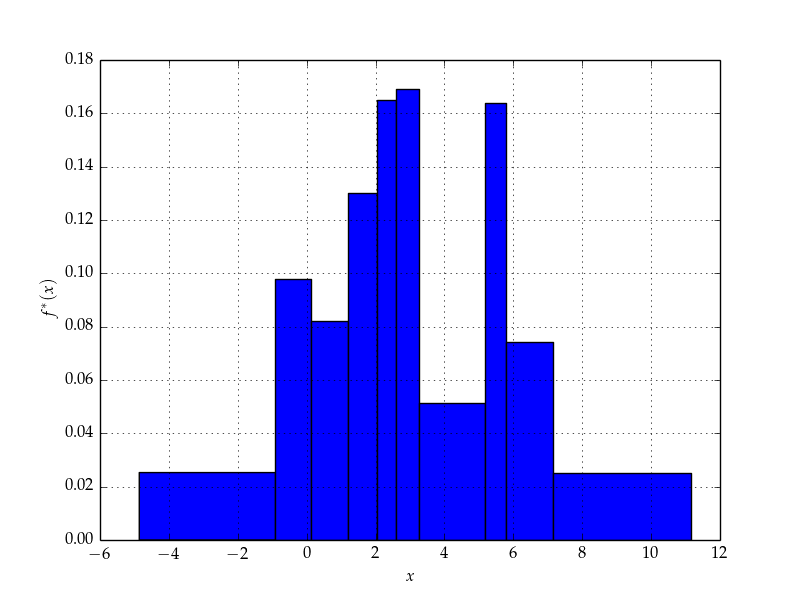
\includegraphics[width=1\linewidth]{pic/stat_series_eq_probability.png}
  \caption{Равновероятностная гистограмма распределения случайной величины $ X $\label{fig:eq-prob_hist}}
\end{figure}

\subsection{Вычисление оценок математического ожидания и дисперсии}

Запишем формулы для расчета cоответствующих оценок:
\begin{equation}
  m^*_X = \overline{x} = \frac{1}{n} \sum_{i=1}^{n} x_i,
\end{equation}

\begin{equation}
  I_\gamma(m_X) = \left[ \overline{x} - z_\gamma \dfrac{S_0}{\sqrt{n}};
    \overline{x} + z_\gamma \dfrac{S_0}{\sqrt{n}} \right],
\end{equation} 

\begin{equation}
  D^*_X = S^2_0 = \frac{1}{n-1} \sum_{i=1}^{n} x^2_i - \frac{n}{n-1} \overline{x}^2,
\end{equation}

\begin{equation}
  I_\gamma(D_X) = \left[ S_0^2 - z_\gamma \sqrt{ \dfrac{2}{n-1}} S_0^2;
    S_0^2 + z_\gamma \sqrt{ \dfrac{2}{n-1}} S_0^2 \right],
\end{equation} 

Результаты вычислений при $ \gamma = 0.95 $:
\begin{equation*}
	\begin{aligned}
		m^*_X &= 2.9967, &
		I_{0.95}(m_X) &= \left[ 2.3605; 3.6329 \right], \\
		D^*_X &= 10.5345, &
                I_{0.95}(D_X) &= \left[ 7.5998; 13.4692 \right].
	\end{aligned}
\end{equation*}

\newpage

\subsection{Выдвижение гипотезы о законе распределения случайной величины $ X $}
По виду графика эмпирической функции распределения $F^*(x)$ и гистограмм выдвинем двухальтернативную
гипотезу о законе распределения случайной величины:

\begin{itemize}
	\item $H_0$ --- величина $X$ распределена по нормальному закону:
	\begin{equation}
          f(x) = f_0(x) = \frac{1}{\sigma\sqrt{2\pi}} \cdot \text{exp} \left[-\frac{(x-m)^2}{2\sigma^2} \right],
	\end{equation}
        \begin{equation}
          F(x) = F_0(x) = 0,5 + \left( \frac{x-m}{\sigma} \right).
        \end{equation}
          
	\item $H_1$ --- величина $X$ не распределена по нормальному закону:
          \begin{align}
		f(x) & \neq f_0(x) ,&
		F(x) & \neq F_0(x).
	\end{align}
\end{itemize}

Учитывая, что $m^* = \overline{x} = 2.9967$ и $\sigma^* = \sqrt{D^*} = 3.2457$, получаем гипотетическую функцию распределения:

\begin{equation*}
  F_0(x) = 0,5 + \Phi \left( \frac{x-\overline{x}}{\sqrt{D^*}} \right) =
  0,5 + \Phi \left( \frac{x- 2.9967}{3.2457} \right)
\end{equation*}

Построим график $F_0(x)$ в одной системе координат с эмпирической функцией распределения $F^*(x)$ (рисунок~\ref{fig:sample_normal}). 

\newpage

\subsection{Проверка гипотезы о нормальном законе распределения 
  случайной величины $ X $ с помощью критерия Пирсона}

Вычислим значение критерия $\chi^2$ на основе равноинтервального статистического ряда
(таблица~\ref{tabl:eq-size_int}) по следующей формуле:
\begin{equation}
  \label{eq:chi^2}
	\chi^2 = n \sum_{j=1}^{10} \frac{(p_j-p^*_j)^2}{p_j}.
\end{equation}

Теоретические вероятности $p_j$ попадания в интервалы равноинтервального статистического ряда нормальной случайной величины с параметрами $m*$, $\sigma^*$ вычислим по следующей формуле:
\begin{equation*}
  p_j = F_0(B_j) - F_0(A_j) = \Phi \left( \frac{B_j + (2.9967)}{3.2457} \right) - \Phi \left( \frac{A_j + (2.9967)}{3.2457} \right).
\end{equation*}

Результаты расчетов приведены в таблице~\ref{tabl:pirson}.

\begin{table}[h!]
  \renewcommand{\arraystretch}{1.2}
  \renewcommand{\tabcolsep}{1.2em}
  \caption{Результаты расчетов значений слагаемых критерия $ \chi^2 $\label{tabl:pirson}}
  \centering
  \small
  \begin{tabular}{|c|c|c|c|c|c|c|c|}
    \hline
    $ j $	& $ A_j $	& $ B_j $	& $ F_0(A_j) $	& $ F_0(B_j) $	& $ p_j $	& $ p_j^{*} $	& $ \frac{(p^{*}_j - p_j)^2}{p_j} $ \\ \hline
1	& $ -\infty $	& -3.259	& 0.0000	& 0.0269	& 0.0269	& 0.0200	& 0.0018 \\ \hline
2	& -3.259	& -1.658	& 0.0269	& 0.0757	& 0.0487	& 0.0500	& 0.0000 \\ \hline
3	& -1.658	& -0.057	& 0.0757	& 0.1732	& 0.0975	& 0.1100	& 0.0016 \\ \hline
4	& -0.057	& 1.544	& 0.1732	& 0.3268	& 0.1536	& 0.1800	& 0.0045 \\ \hline
5	& 1.544	& 3.145	& 0.3268	& 0.5188	& 0.1921	& 0.2000	& 0.0003 \\ \hline
6	& 3.145	& 4.746	& 0.5188	& 0.7055	& 0.1866	& 0.0900	& 0.0500 \\ \hline
7	& 4.746	& 6.347	& 0.7055	& 0.8492	& 0.1438	& 0.1900	& 0.0149 \\ \hline
8	& 6.347	& 7.948	& 0.8492	& 0.9365	& 0.0873	& 0.1100	& 0.0059 \\ \hline
9	& 7.948	& 9.549	& 0.9365	& 0.9783	& 0.0418	& 0.0300	& 0.0033 \\ \hline
10	& 9.549	& $ +\infty $	& 0.9783	& 1.0000	& 0.0217	& 0.0200	& 0.0001 \\ \hline
	&	&	&	&Всего:	&1.0000	&1.0000	&0.0826 \\ \hline

  \end{tabular}
\end{table}

Проверим выполнение контрольного соотношения для $p_j$:
\begin{align}
	\left| 1 - \sum_{j=1}^{10} p_j \right| = value \le 0.01.
\end{align}

В cоответствии с формулой~\eqref{eq:chi^2} получаем $\chi^2= 100 \cdot 0.0826 = $ j $	& $ A_j $	& $ B_j $	& $ F_0(A_j) $	& $ F_0(B_j) $	& $ p_j $	& $ p_j^{*} $	& $ \frac{(p^{*}_j - p_j)^2}{p_j} $ \\ \hline
1	& $ -\infty $	& -3.259	& 0.0000	& 0.0269	& 0.0269	& 0.0200	& 0.0018 \\ \hline
2	& -3.259	& -1.658	& 0.0269	& 0.0757	& 0.0487	& 0.0500	& 0.0000 \\ \hline
3	& -1.658	& -0.057	& 0.0757	& 0.1732	& 0.0975	& 0.1100	& 0.0016 \\ \hline
4	& -0.057	& 1.544	& 0.1732	& 0.3268	& 0.1536	& 0.1800	& 0.0045 \\ \hline
5	& 1.544	& 3.145	& 0.3268	& 0.5188	& 0.1921	& 0.2000	& 0.0003 \\ \hline
6	& 3.145	& 4.746	& 0.5188	& 0.7055	& 0.1866	& 0.0900	& 0.0500 \\ \hline
7	& 4.746	& 6.347	& 0.7055	& 0.8492	& 0.1438	& 0.1900	& 0.0149 \\ \hline
8	& 6.347	& 7.948	& 0.8492	& 0.9365	& 0.0873	& 0.1100	& 0.0059 \\ \hline
9	& 7.948	& 9.549	& 0.9365	& 0.9783	& 0.0418	& 0.0300	& 0.0033 \\ \hline
10	& 9.549	& $ +\infty $	& 0.9783	& 1.0000	& 0.0217	& 0.0200	& 0.0001 \\ \hline
	&	&	&	&Всего:	&1.0000	&1.0000	&0.0826 \\ \hline
 $.

Вычислим число степеней свободы: $ k = M - 1 - s = 10 - 1 - 2 = 7 $. 

По заданному уровню значимости ($\alpha = 0,05$) из таблицы распределения $\chi^2$ выбирем критическое значение:
\begin{equation*}
  \chi^2_{\alpha; k} = \chi^2_{0.05; 7} = 14.07.
\end{equation*}

\textbf{Вывод:} так как $\chi^2 = $ j $	& $ A_j $	& $ B_j $	& $ F_0(A_j) $	& $ F_0(B_j) $	& $ p_j $	& $ p_j^{*} $	& $ \frac{(p^{*}_j - p_j)^2}{p_j} $ \\ \hline
1	& $ -\infty $	& -3.259	& 0.0000	& 0.0269	& 0.0269	& 0.0200	& 0.0018 \\ \hline
2	& -3.259	& -1.658	& 0.0269	& 0.0757	& 0.0487	& 0.0500	& 0.0000 \\ \hline
3	& -1.658	& -0.057	& 0.0757	& 0.1732	& 0.0975	& 0.1100	& 0.0016 \\ \hline
4	& -0.057	& 1.544	& 0.1732	& 0.3268	& 0.1536	& 0.1800	& 0.0045 \\ \hline
5	& 1.544	& 3.145	& 0.3268	& 0.5188	& 0.1921	& 0.2000	& 0.0003 \\ \hline
6	& 3.145	& 4.746	& 0.5188	& 0.7055	& 0.1866	& 0.0900	& 0.0500 \\ \hline
7	& 4.746	& 6.347	& 0.7055	& 0.8492	& 0.1438	& 0.1900	& 0.0149 \\ \hline
8	& 6.347	& 7.948	& 0.8492	& 0.9365	& 0.0873	& 0.1100	& 0.0059 \\ \hline
9	& 7.948	& 9.549	& 0.9365	& 0.9783	& 0.0418	& 0.0300	& 0.0033 \\ \hline
10	& 9.549	& $ +\infty $	& 0.9783	& 1.0000	& 0.0217	& 0.0200	& 0.0001 \\ \hline
	&	&	&	&Всего:	&1.0000	&1.0000	&0.0826 \\ \hline
 {<}sign{>} \chi^2_{0,05;7} $, то гипотеза $H_0$ о нормальном законе распределения принимается (отклоняется). 


\subsection{Проверка гипотезы о нормальном законе распределения 
  случайной величины $ X $ с помощью критерия Колмогорова}

По рисунку~\ref{fig:sample_normal} определим максимальное по модулю отклонение между функциями $F^*(x)$ и $F_0(x)$:
\begin{align}
	Z = \max_{i=1}^n \Big| F^*(x_i) - F_0(x_i) \Big| = value.
\end{align}

Вычислим значение критерия Колмогорова по формуле:
\begin{align}
  \lambda &= \sqrt{n} \cdot Z, \\ \nonumber
  \lambda &= \sqrt{100} \cdot 0.0777 = 0.7767.
\end{align}

Из таблицы <<критических значений>> для критерия Колмогорова по заданному уровню значимости ($\alpha = 0.05$)
выбираем критическое значение $\lambda_{\gamma} = \lambda_{1-\alpha} = \lambda_{0.95} = 1.36 $.

\textbf{Вывод:} так как $\lambda = 0.7767 {<}notation{>} \lambda_{0,95} $, то гипотеза $H_0$ о нормальном законе распределения принимается (отклоняется).

\newpage
\fancyhf{}
\newgeometry{left=1cm,right=1cm,top=1cm}
\begin{landscape}
  \begin{figure}[H]
    \centering
    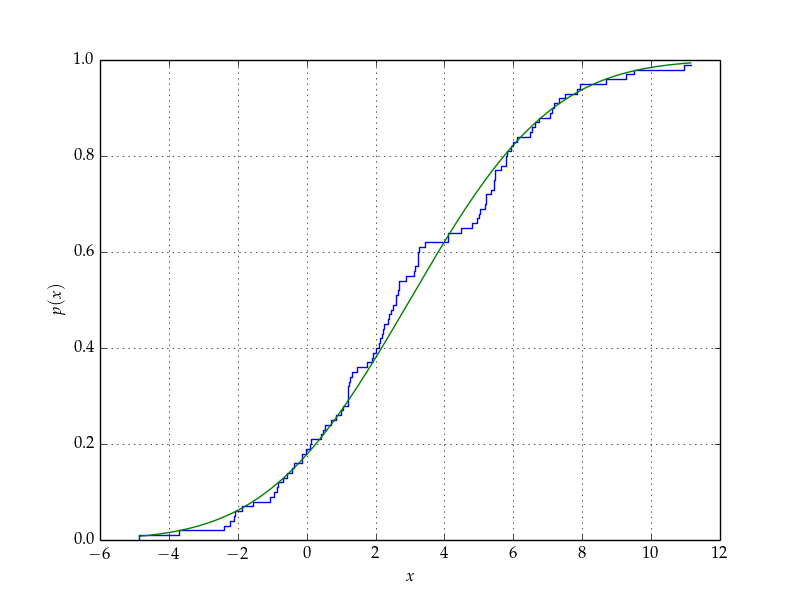
\includegraphics[width=0.9\linewidth]{pic/sample_normal.png}
    \caption{График гипотетической и эмпирической функций распределения случайной величины $ X $\label{fig:sample_normal}}
  \end{figure}
\end{landscape}
\restoregeometry

\end{document}